% LaTeX layout by Jonas Kahler, jonas@derkahler.de
% AutoTux Final Report
% Group Tux:
% Max Enelund, Jerker Ersare, Thorsteinn D. Jörundsson,
% Jonas Kahler, Dennis Karlberg Niklas le Comte, Marco Trifance, Ivo Vryashkov
% Chapter 6 - Hardware and Software Integration
\chapter[Hardware and Software Integration]{Hardware and\\Software Integration}
%% Low-level Board
\section[Low-level Board]{Low-level Board\textsuperscript{[JE \& TDJ]}}
\begin{figure}[ht]
  \centering
  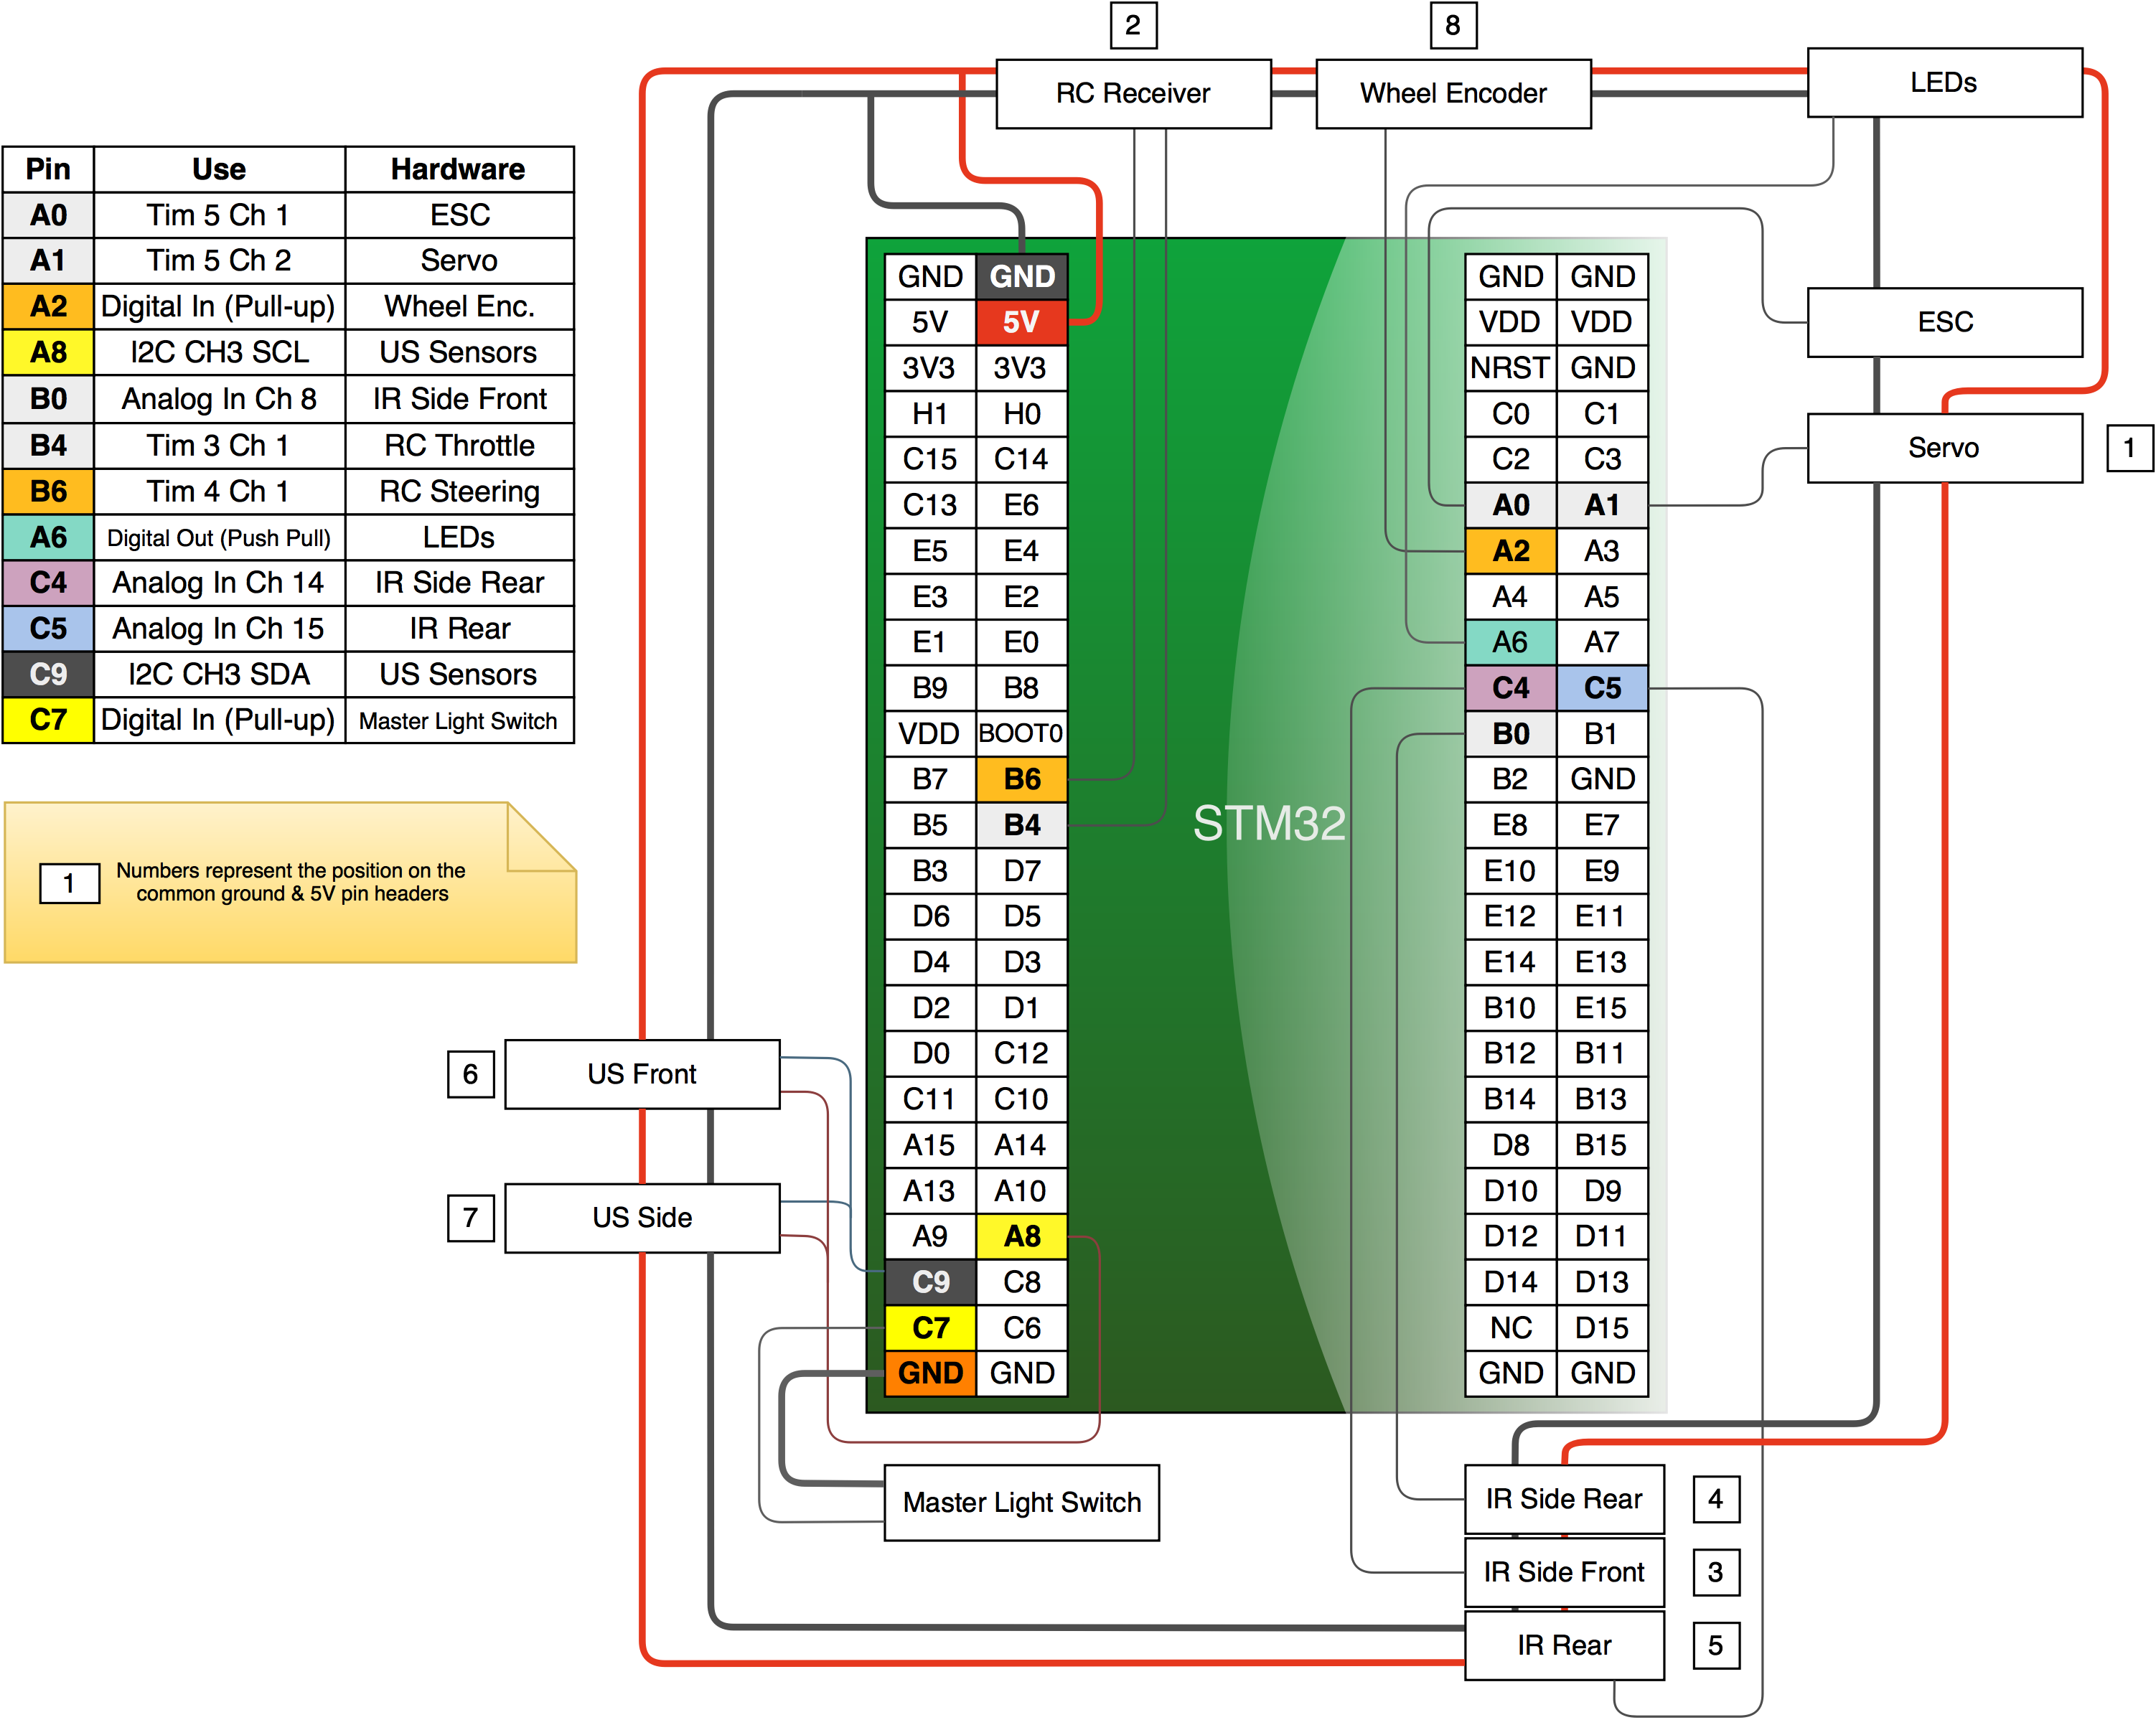
\includegraphics[width=1\textwidth]{X-STM32BlockDiagram.png}
  \caption{Wiring Schematic (Block diagram)}
  \label{blockdiag}
\end{figure}
\textsuperscript{\textbf{[JE]}}
It took a while for us to arrive at this wiring solution. Our decisions were
limited by which STM32 pins support which features, and which features and pins
can be used simultaneously. For example, one thing we learned along the way was
that PWM output is most easily set up with the so called ``general purpose''
timers, numbered 2 to 5, on the STM32. These timers are connected to a certain
set of pins. Another example of differences between pins is that some tolerate
only 3.3V instead of 5V. We had to refer to the user manual of the STM32
continuously when deciding where to connect each new hardware component type.\\

\noindent
The master light switch is an on/off switch that when turned off will cause the
light controlling module to turn all lights off. This is helpful to save battery
power when lights are not needed.\\

\noindent
For most hardware interaction we use the drivers provided by ChibiOS:
\begin{itemize}
   \item The PWM (Pulse Width Modulation) driver for generating PWM output to
       control the ESC and servo
   \item The ICU (Input Capture Unit) driver for measurement of incoming RC PWM
       signal
   \item The I\textsuperscript{2}C (Inter-Integrated Circuit) driver for
       interacting with the ultrasonic sensors
   \item The ADC (Analog-to-Digital Converter) driver for reading the analog
       values from the infrared sensors
   \item The EXT (External) driver to execute a callback when the wheel encoder
       signal goes (digital) high.
\end{itemize}
However, since the neopixel light strips doesn’t use a very common communication
protocol for their digital signal, there are no drivers for it provided by
ChibiOS. We evaluated third-party drivers but found only one somewhat viable
option, that happened to require two of the STM32’s timers. Eventually we
decided to write our own software based bit-banging driver instead, explained
further in the Implementation section \textbf{[JONAS MAKE LINK]}.\\

\noindent
As discussed in the Software Architecture section \textbf{[JONAS MAKE LINK]},
some of the hardware modules for sensor input (wheel encoder, RC input) have
interrupt callback functions that automatically gets executed whenever values
change. Others (ultrasonic and infrared) need to initiate the measurement on the
main thread, running at a frequency of 13.8 Hz. For the infrared ADC
measurement, a callback is then executed automatically when the conversion is
finished.\\

\noindent
The frequency of 13.8 Hz is somewhat limited by our ultrasonic sensors, that
need at least 65 ms to complete their ranging. This means a call is first made
to start ranging, and a while later a call is made to fetch the measured values.
It may have been possible to decrease the time needed by adjusting the range
settings of the ultrasonic sensors, which could have been interesting to explore
if the project would continue for a longer time.\\

\noindent
Most hardware and software integration worked well and was straightforward. The
most problematic hardware components were the ultrasonic sensors, where the
I\textsuperscript{2}C communication seems sensitive to fluctuations in voltage,
which can occur for example when the steering servo is used. We reduced this
sensitivity by mounting external pull-up resistors connected to the
I\textsuperscript{2}C bus.\\

\noindent
Another problem was interference between the two sensors: the signal of one
sensor would be perceived by the other sensors as a reflected sound, and
therefore lower the measured distances of both sensors compared to if they were
running alone. We handled this problem by reducing the gain of both sensors,
making them send out weaker signals. This problem may not have had the same
impact if the I\textsuperscript{2}C driver on ChibiOS supported broadcast mode,
i.e. the possibility of sending a request to both sensors at the exact same to
start their ranging process.\\

\noindent
\textsuperscript{\textbf{[TDJ]}}
We also ran into issues with faulty hardware, most notably the front-right
ultrasonic sensor and the side-rear infrared sensor. While troubleshooting the
ultrasonic sensor, we noted that it seemingly worked as intended while being run
on an Arduino microcontroller as opposed to the STM32.\\

\noindent
The ultrasonic sensor was replaced with a sensor from another group which had an
Arduino low-level board. The replacement sensor worked as intended, but they
returned our original sensor as it became unstable after a short period of use
on the Arduino. The faulty sensor was then returned to Federico and a new one
was installed which worked as intended.\\

\noindent
The faulty side-rear IR sensor received wildly fluctuating values and tiny
adjustments to its wiring would cause further disruption, and would at times
cause the STM32 to power off. We noted that this was still the case after
replacing its wiring, leading us to believe that this was either a soldering
issue or a problem with the sensor itself. Slight adjustments to the sensor
could cause it to function normally, but these adjustments were temporary at
best and the smallest interruptions to it would revert the sensor to its
previous broken state.\\

\noindent
A replacement sensor was acquired, and the original wiring was kept in place.
The new sensor gave consistent values and did not cause any interruptions to the
STM32.
\begin{figure}[ht]
  \centering
  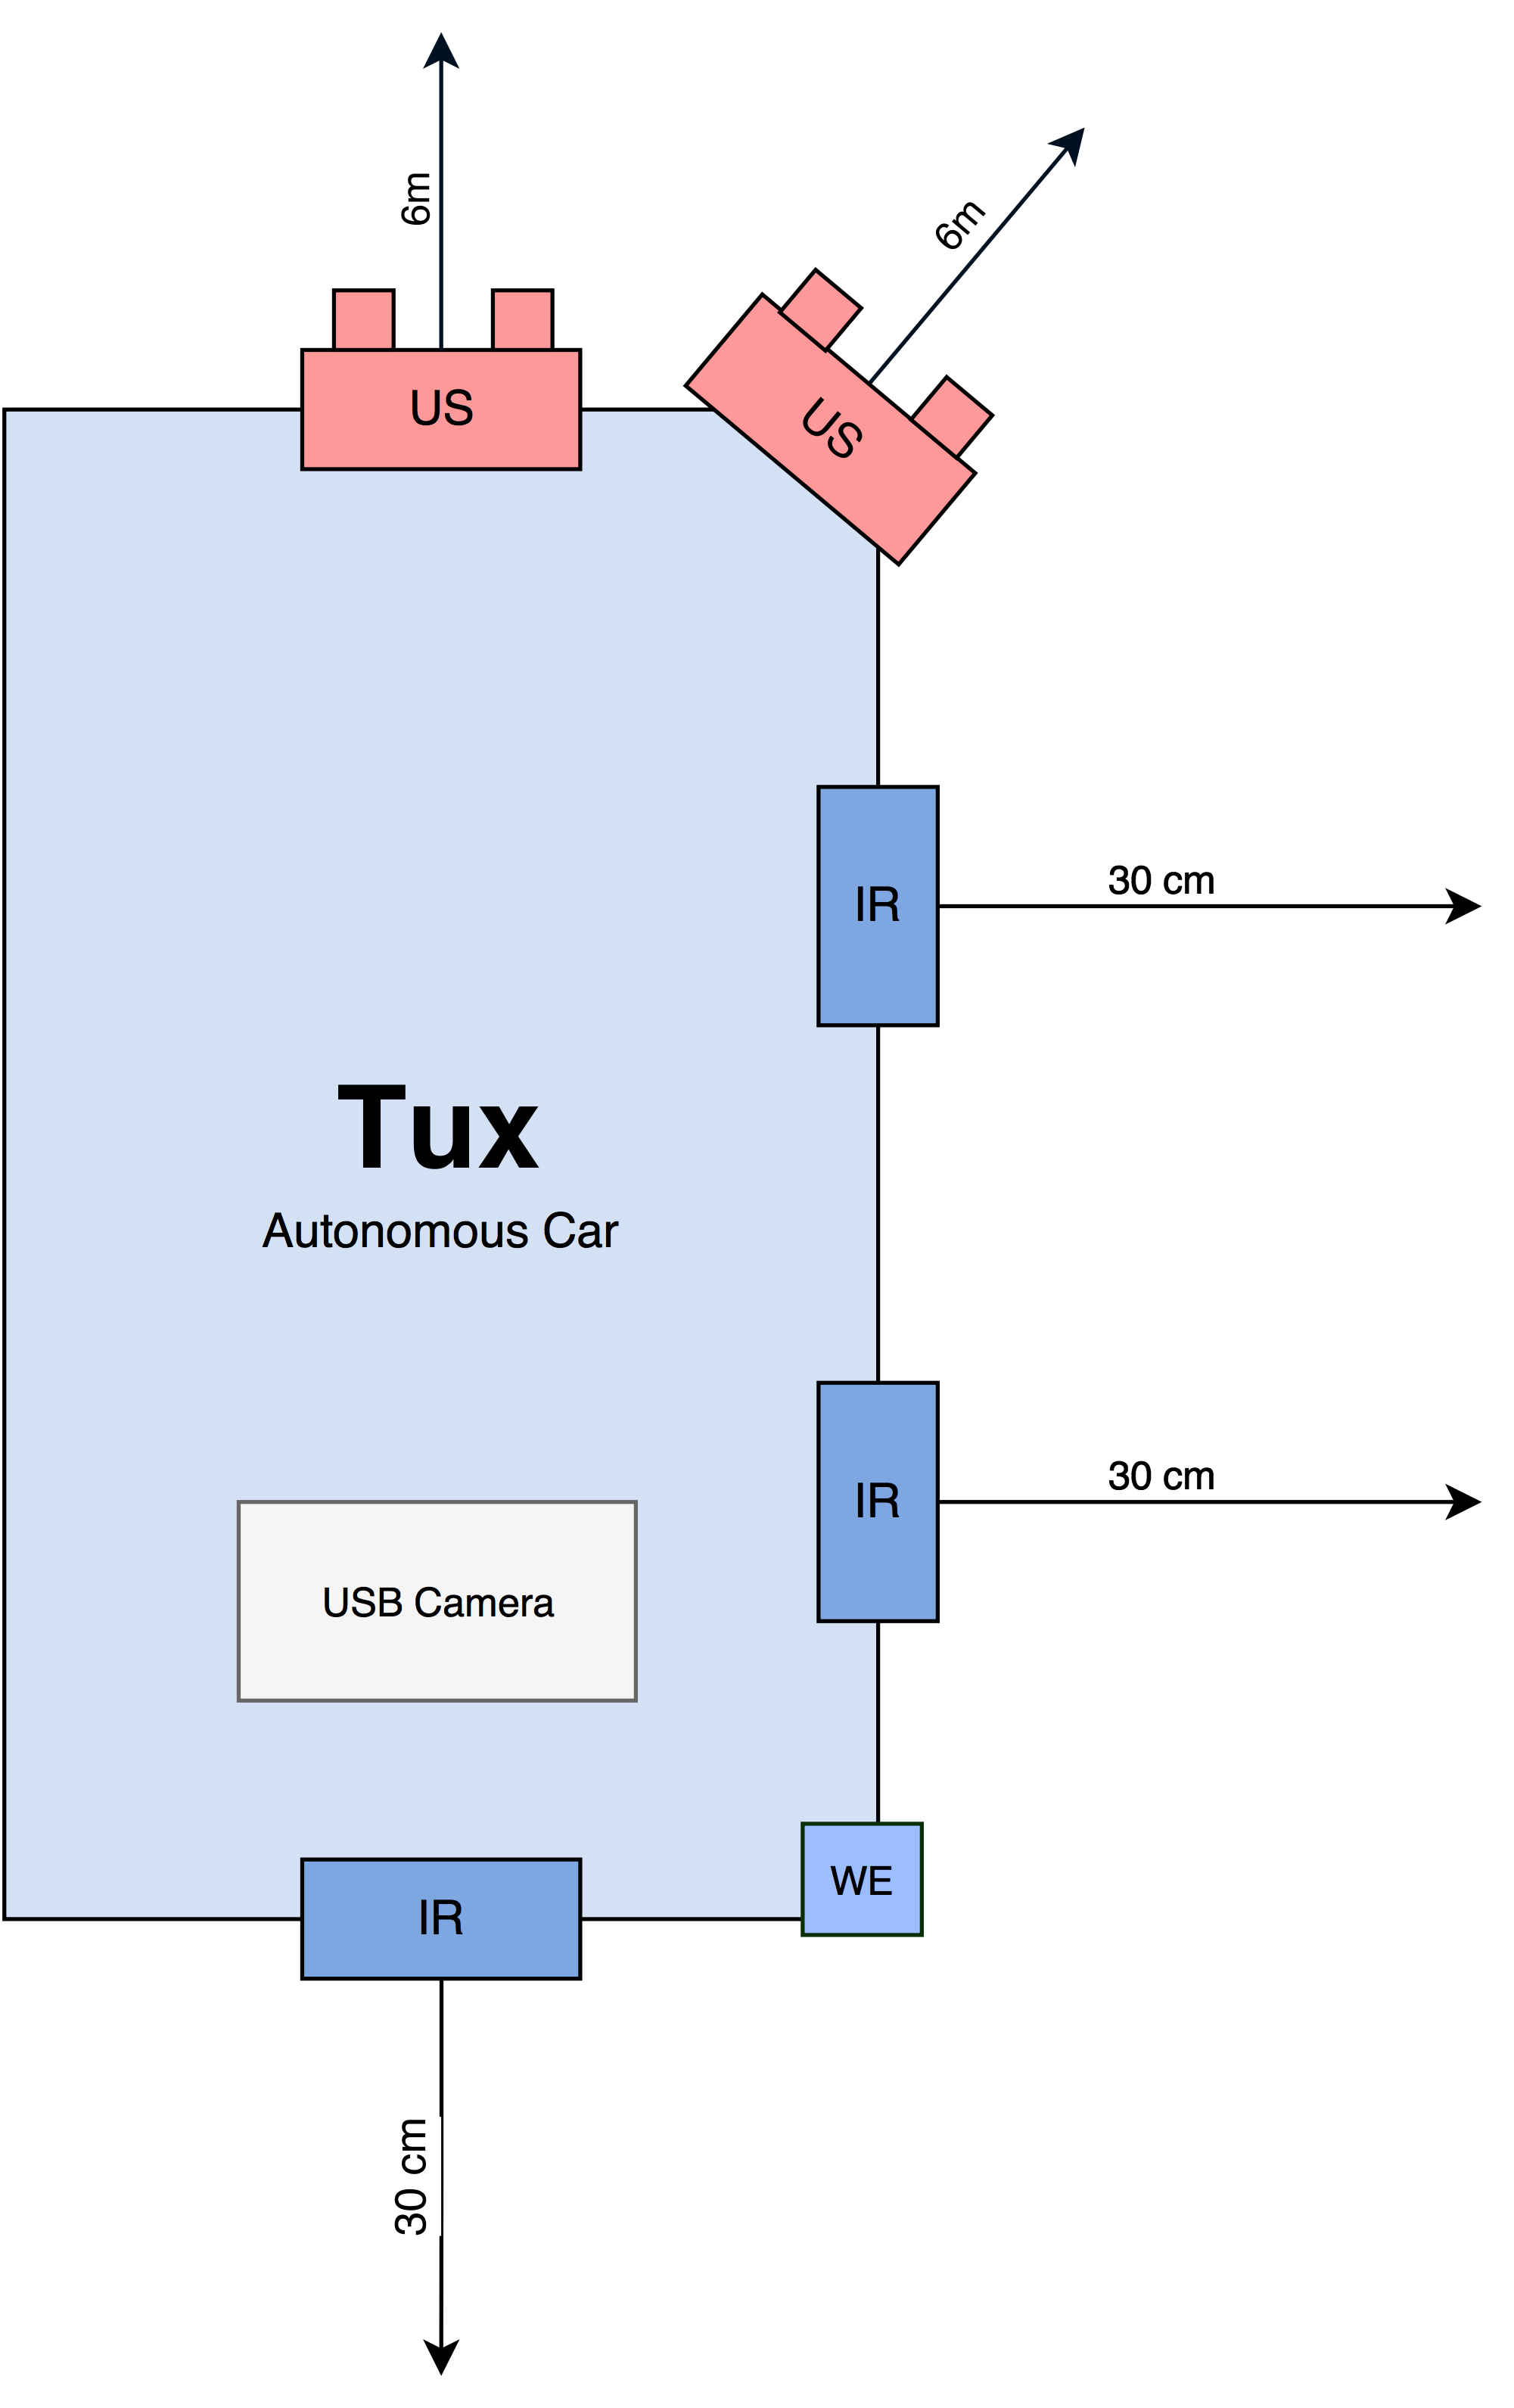
\includegraphics[height=18cm]{X-BirdsEyeSensorDiagram.png}
  \caption{Sensor layout}
  \label{sensorlay}
\end{figure}
